\documentclass[10pt,twocolumn,letterpaper]{article}

\usepackage[margin=0.75in,columnsep=0.3in]{geometry}
\usepackage{times}
\usepackage[T1]{fontenc}
\usepackage[utf8]{inputenc}
\usepackage{amsmath,amssymb}
\usepackage{graphicx}
\usepackage{booktabs}
\usepackage{multirow}
\usepackage{xcolor}
\usepackage{colortbl}
\usepackage{tikz}
\usetikzlibrary{arrows.meta,positioning,decorations.pathreplacing,calc}
\usepackage{caption}
\captionsetup{font=small,labelfont=bf}
\usepackage[hidelinks]{hyperref}
\usepackage{cleveref}

\newcommand{\best}[1]{\textbf{\textcolor{red!75!black}{#1}}}
\newcommand{\second}[1]{\underline{\textcolor{blue!70!black}{#1}}}
\newcommand{\ours}{\cellcolor{gray!12}}

\newcommand{\gainBalStream}{+0.41}
\newcommand{\gainQualStream}{+0.49}
\newcommand{\gainEfStream}{-0.19}
\newcommand{\gainBalClean}{-0.34}
\newcommand{\gainQualClean}{-0.22}
\newcommand{\gainEfClean}{-1.28}
\newcommand{\nClips}{182}
\newcommand{\nFrames}{1{,}092}
\newcommand{\codecBest}{AV1 (SVT)}
\newcommand{\vmafQualStream}{+3.0}
\newcommand{\vmafBalStream}{+1.9}


\title{\textbf{LiveActionSR: Tiny Real-Time Super-Resolution for Streamed Live-Action Video in the Browser}}
\author{PianoNic\\{\small\url{https://github.com/PianoNic/LiveActionSR}}}
\date{November 2026}

\begin{document}
\maketitle

\begin{abstract}
Upscaling in the video player has to fit a few milliseconds per frame on whatever GPU the viewer
has, and the frames it sees are not clean downscales but H.264, HEVC or AV1 decodes. Shader
networks that fit that budget exist, but the good ones are trained on anime and the
content-neutral ones are LGPL. We present \emph{LiveActionSR}, two 2$\times$ luma networks of
12k and 48k parameters, trained only on permissively licensed live-action footage that we push
through real x264, x265 and SVT-AV1 round-trips. They run as hand-written WGSL compute shaders in
a browser video player, in 2.9 and 9.9\,ms for 1080p$\to$4K on a desktop GPU and about a
third of that for 720p$\to$1440p. On held-out streaming-compressed clips they gain
\gainBalStream\,dB and \gainQualStream\,dB PSNR-Y (\vmafBalStream\ and \vmafQualStream\ VMAF) over
Lanczos. Under the same protocol a ten times larger network fine-tuned for streaming, EfRLFN, stays
below Lanczos. On clean downscales the picture splits: our networks gain up to
0.6\,dB on textured frames but lose on flat, nearly flawless ones, ending
\gainQualClean\,dB below Lanczos on average. Doubling the training data raised both gains on every
validation set. We release the weights (MIT), the training pipeline, the
data recipe with its licence audit, and a WebGPU port of EfRLFN.
\end{abstract}

\section{Introduction}

Most films and series reach viewers as 720p or 1080p streams on screens with more pixels.
Players upscale with a bilinear or bicubic filter, and the picture they start from has already
lost texture to the encoder. A learned upscaler can do better, but a player-side one has three
constraints that offline video SR does not have:

\begin{enumerate}
\setlength\itemsep{0pt}
\item \textbf{Budget.} The upscaler shares the frame interval with decoding and compositing, on
integrated GPUs as well as discrete ones. Our target is a few milliseconds at 1080p output.
\item \textbf{Degradation.} The input is a codec decode. Blocking, banding and smeared texture
dominate, and sharpening them makes them worse.
\item \textbf{Licence.} The weights ship inside a web page, so every training source has to allow
commercial reuse and machine learning.
\end{enumerate}

The mpv shader ecosystem covers the first constraint well. But ArtCNN, CuNNy and Anime4K are
trained on anime or visual novels, and the content-neutral RAVU, NNEDI3 and FSRCNNX are LGPL-3.0.
Real-time research models such as SPAN~\cite{span} or RLFN~\cite{rlfn} are trained on clean
bicubic downscales (DIV2K) and run in PyTorch or TensorRT, not in browser shaders. EfRLFN~\cite{efrlfn} targets exactly streaming content, but at 487k
parameters it runs in real time only for SD sources.

LiveActionSR takes the opposite trade. We keep the network to a straight stack of 3$\times$3
convolutions on luma, which a browser can run in one fused pass per layer, and put the effort into
the data: \textbf{75k} training pairs from \textbf{67} scenes in five permissively licensed
collections, each degraded through a sampled codec round-trip. Our contributions:

\begin{itemize}
\setlength\itemsep{0pt}
\item two MIT-licensed 2$\times$ networks (12k and 48k parameters) for compressed live action, with
the plugin that runs them on WebGPU (\cref{sec:runtime});
\item a reproducible data recipe that reads only the sampled positions of large masters with HTTP
range requests, with a source-by-source licence audit (\cref{sec:data});
\item a two-track benchmark, clean and streaming, against interpolation and EfRLFN
(\cref{sec:exp});
\item a WebGPU port of EfRLFN through a small graph format, released as a separate preset.
\end{itemize}

\begin{figure*}[t]
  \centering
  \resizebox{0.86\textwidth}{!}{% LiveActionSR-2x architecture in the PlotNeuralNet look: feature maps as 3D boxes whose depth is
% the channel count and whose face is the spatial size. Plain TikZ, no external layer files.
\begin{tikzpicture}[x=1cm,y=1cm,
    conn/.style={-{Stealth[length=2.2mm]}, line width=0.9pt, draw=edge},
    lbl/.style={font=\scriptsize, align=center},
    cap/.style={font=\scriptsize\bfseries, align=center}]
  \definecolor{conv}{RGB}{255,215,140}
  \definecolor{relu}{RGB}{235,150,70}
  \definecolor{shuf}{RGB}{160,200,235}
  \definecolor{inp}{RGB}{200,200,200}
  \definecolor{outp}{RGB}{170,220,170}
  \definecolor{edge}{RGB}{70,80,100}

  % \fmap{x}{w(face width)}{h(face height)}{d(depth along the oblique axis)}{fill}{name}
  \newcommand{\fmap}[6]{%
    \coordinate (#6-sw) at (#1,-#3/2);
    \fill[#5, draw=black!70, line width=0.35pt] (#1,-#3/2) rectangle ++(#2,#3);
    \fill[#5!75!black, draw=black!70, line width=0.35pt]
      (#1+#2,-#3/2) -- ++(#4*0.5,#4*0.35) -- ++(0,#3) -- ++(-#4*0.5,-#4*0.35) -- cycle;
    \fill[#5!88!white, draw=black!70, line width=0.35pt]
      (#1,#3/2) -- ++(#4*0.5,#4*0.35) -- ++(#2,0) -- ++(-#4*0.5,-#4*0.35) -- cycle;
    \coordinate (#6-w) at (#1,0);
    \coordinate (#6-e) at (#1+#2+#4*0.25,#4*0.175);
    \coordinate (#6-n) at (#1+#2/2+#4*0.25,#3/2+#4*0.35);
    \coordinate (#6-s) at (#1+#2/2,-#3/2);
  }

  % input luma
  \fmap{0}{0.12}{2.0}{0.25}{inp}{in}
  \node[cap, below=2pt] at (in-s) {$Y$\\$H\times W$};

  % conv1 + ReLU
  \fmap{1.0}{0.25}{2.0}{1.6}{conv}{c1}
  \fill[relu, draw=black!70, line width=0.35pt] (1.25,-1.0) rectangle ++(0.08,2.0);
  \node[cap, below=2pt] at (c1-s) {conv 3$\times$3\\$1\to C$};

  % 5 hidden conv + ReLU blocks
  \foreach \i in {0,...,4} {
    \pgfmathsetmacro{\xx}{2.55+0.78*\i}
    \fmap{\xx}{0.25}{2.0}{1.6}{conv}{h\i}
    \fill[relu, draw=black!70, line width=0.35pt] (\xx+0.25,-1.0) rectangle ++(0.08,2.0);
  }
  \draw[decorate, decoration={brace, amplitude=4pt, mirror}] (2.55,-1.25) -- (6.0,-1.25)
    node[midway, below=5pt, cap] {5 $\times$ [conv 3$\times$3, $C\to C$, ReLU]};

  % conv to 4 channels
  \fmap{6.95}{0.25}{2.0}{0.4}{conv}{c4}
  \node[cap, below=2pt] at (c4-s) {conv 3$\times$3\\$C\to 4$};

  % depth to space
  \fmap{8.15}{0.12}{4.0}{0.25}{shuf}{ds}
  \node[cap, below=2pt] at (ds-s) {depth-to-space\\$2H\times 2W$};

  % sum and output
  \node[circle, draw=black!70, fill=white, inner sep=1.5pt, font=\small] (sum) at (9.35,0) {$+$};
  \fmap{10.0}{0.12}{4.0}{0.25}{outp}{out}
  \node[cap, below=2pt] at (out-s) {$\hat Y$, clamp $[0,1]$\\$2H\times 2W$};

  \draw[conn] (in-e) -- (c1-w);
  \draw[conn] (c1-e) -- (h0-w);
  \draw[conn] (h4-e) -- (c4-w);
  \draw[conn] (c4-e) -- (ds-w);
  \draw[conn] (ds-e) -- (sum);
  \draw[conn] (sum) -- (out-w);

  % bilinear residual
  \draw[conn, rounded corners=6pt] (in-n) -- ++(0,0.85) -| node[pos=0.25, above, lbl]
    {bilinear $2\times$ (half-pixel centres, clamp-to-edge)} (sum.north);

  \node[lbl, anchor=west] at (0.0,-2.75) {$C=16$: \textit{balanced}, 12{,}340 parameters \quad
    $C=32$: \textit{quality}, 47{,}716 parameters \quad all convolutions pad by replication};
\end{tikzpicture}
}
  \caption{\textbf{LiveActionSR-2x.} A plain chain of 3$\times$3 convolutions on the luma plane
  predicts a residual over a bilinear 2$\times$ upscale; depth-to-space~\cite{espcn} turns 4
  channels into the 2$\times$ grid. Chroma is upscaled bilinearly. The chain maps one-to-one onto
  WGSL compute passes.}
  \label{fig:arch}
\end{figure*}

\section{Related work}

\paragraph{Efficient SR.} SRCNN~\cite{srcnn} and FSRCNN~\cite{fsrcnn} established small
convolutional SR. ESPCN~\cite{espcn} moved the upsampling to the end with a sub-pixel
convolution, which we use. The NTIRE efficient SR challenges~\cite{ntire24} drove networks such
as RLFN~\cite{rlfn} and SPAN~\cite{span} to a few hundred thousand parameters, but they rank on
clean DIV2K bicubic downscales and desktop runtimes in PyTorch.

\paragraph{Compressed video SR.} Blind degradation models~\cite{bsrgan,realesrgan} add JPEG and
noise to the synthesis. The AIM 2024 challenge~\cite{aim24} targets AV1-compressed content and
shows that VMAF rewards sharpening even when PSNR drops. EfRLFN~\cite{efrlfn} benchmarks
real-time SR on streaming content and fine-tunes an RLFN variant with efficient channel
attention~\cite{eca} on it. It is our main external reference.

\paragraph{Shader upscalers.} AMD FSR~1~\cite{fsr} (EASU + RCAS) and NVIDIA NIS are MIT and very
cheap, but not learned. Anime4K~\cite{anime4k} and ArtCNN~\cite{artcnn} are learned shader CNNs
for anime. To our knowledge no small, permissively licensed shader network targets compressed
live action.

\section{Method}

\subsection{Network}
\Cref{fig:arch} shows the network. Given the BT.709 luma $Y\in[0,1]^{H\times W}$ of a decoded frame,
\begin{equation}
\hat Y = \mathrm{clamp}_{[0,1]}\big(\mathcal{B}_{2}(Y) + \mathrm{D2S}(f_\theta(Y))\big),
\end{equation}
where $\mathcal{B}_2$ is bilinear 2$\times$ upsampling with half-pixel centres, $f_\theta$ is seven
3$\times$3 convolutions ($1\to C$, five times $C\to C$, $C\to4$) with ReLU in between, and D2S is
depth-to-space. Every convolution pads by replicating the edge, so the borders match the shader.
\emph{balanced} uses $C=16$ (12{,}340 parameters, 12.3k MACs per source pixel) and \emph{quality}
$C=32$ (47{,}716, 47.6k MACs). The networks are trained on luma only: chroma carries little detail
after 4:2:0 subsampling, and one input channel cuts the cost of the first and last layers.

\subsection{Browser runtime}
\label{sec:runtime}
The plugin copies each decoded frame into a texture with \texttt{requestVideoFrameCallback} and
\texttt{copyExternalImageToTexture}, then runs a chain of WGSL compute passes:
\begin{enumerate}
\setlength\itemsep{0pt}
\item a deband in the style of f3kdb;
\item the CNN, if the screen is more than 1.2$\times$ the video;
\item FSR~1 EASU for any remaining scale;
\item RCAS at reduced strength;
\item luma film grain.
\end{enumerate}
Each convolution is one compute dispatch. One invocation produces four output channels of one
pixel, reads its 3$\times$3$\times$C neighbourhood from an \texttt{rgba16float} texture array, and
accumulates in f32 with f16 storage when \texttt{shader-f16} is available.

An \emph{auto} mode measures every preset on the actual video and screen and picks the strongest
that fits $\min(12\,\mathrm{ms}, 0.35\cdot\Delta t_{\mathrm{frame}})$. It steps down at run time
when frames drop. HDR (PQ/HLG) sources are drawn through a 2D canvas first, so they get the
browser's tone mapping before upscaling.

\section{Data}
\label{sec:data}

\begin{figure}[t]
  \centering
  \resizebox{\columnwidth}{!}{% Data and deployment pipeline.
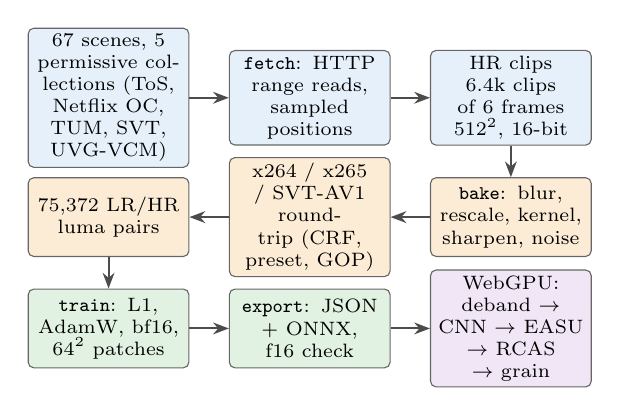
\begin{tikzpicture}[
    node distance=4mm and 5mm,
    box/.style={draw=black!60, rounded corners=2pt, fill=#1, align=center, font=\scriptsize,
                minimum height=10mm, text width=19mm, inner sep=2pt},
    box/.default=white,
    arr/.style={-{Stealth[length=2mm]}, line width=0.7pt, draw=black!70},
    grp/.style={draw=black!35, dashed, rounded corners=3pt, inner sep=3pt},
    gl/.style={font=\scriptsize\itshape, text=black!60}]
  \definecolor{c1}{RGB}{230,240,250}
  \definecolor{c2}{RGB}{252,236,214}
  \definecolor{c3}{RGB}{226,242,226}
  \definecolor{c4}{RGB}{240,230,245}

  \node[box=c1] (src) {67 scenes, 5 permissive collections (ToS, Netflix OC, TUM, SVT, UVG-VCM)};
  \node[box=c1, right=of src] (fetch) {\texttt{fetch}: HTTP range reads, sampled positions};
  \node[box=c1, right=of fetch] (hr) {HR clips\\6.4k clips of 6 frames\\512$^2$, 16-bit};

  \node[box=c2, below=of hr] (deg) {\texttt{bake}: blur, rescale, kernel, sharpen, noise};
  \node[box=c2, left=of deg] (codec) {x264 / x265 / SVT-AV1 round-trip (CRF, preset, GOP)};
  \node[box=c2, left=of codec] (pairs) {75{,}372 LR/HR luma pairs};

  \node[box=c3, below=of pairs] (train) {\texttt{train}: L1, AdamW, bf16, 64$^2$ patches};
  \node[box=c3, right=of train] (export) {\texttt{export}: JSON + ONNX, f16 check};
  \node[box=c4, right=of export] (gpu) {WebGPU: deband $\to$ CNN $\to$ EASU $\to$ RCAS $\to$ grain};

  \draw[arr] (src) -- (fetch);
  \draw[arr] (fetch) -- (hr);
  \draw[arr] (hr) -- (deg);
  \draw[arr] (deg) -- (codec);
  \draw[arr] (codec) -- (pairs);
  \draw[arr] (pairs) -- (train);
  \draw[arr] (train) -- (export);
  \draw[arr] (export) -- (gpu);
\end{tikzpicture}
}
  \caption{\textbf{Pipeline.} Positions are sampled in the masters and only those bytes are
  fetched; every HR clip is degraded four times with sampled parameters and a real encoder
  round-trip.}
  \label{fig:pipeline}
\end{figure}

\paragraph{Sources.} We only use footage whose terms allow commercial reuse, derivatives and
machine learning (\cref{tab:data}). Netflix Open Content~\cite{netflixoc} provides cinema-grade
masters: \emph{Chimera}, \emph{El Fuente}, \emph{Meridian}, \emph{Nocturne} and \emph{Sparks}. Its
older CC BY-NC-ND notices were replaced by CC BY 4.0 files across the bucket in 2021, which we
verified file by file. UVG-VCM~\cite{uvgvcm} adds 4K60 sports, traffic and indoor scenes; Tears of
Steel, the TUM and the SVT test sequences complete the set. We rejected the stock sites (Pexels,
Pixabay, Unsplash, Mixkit, Videvo, Coverr), because their terms forbid ML use or bulk download,
and every NC or ND dataset.

\paragraph{Sampling.} Masters range from 1080p PNG sequences to 46\,GB ProRes files and 53\,GB raw
16-bit YUV. \texttt{fetch} reads only what it needs:
\begin{itemize}
\setlength\itemsep{0pt}
\item for raw YUV, a band of rows at each sampled frame;
\item for zipped JPEG 2000 sequences, the selected members via the central directory;
\item for ProRes, ffmpeg seeks over HTTP.
\end{itemize}
It stores deduplicated 512$\times$512 crops of 6 frames in 16-bit PNG. The Meridian PQ/P3 master is
tone-mapped to BT.709. Whole scenes are held out for validation.

\paragraph{Degradation.} Each HR clip yields four training variants. The sampled steps are:
\begin{itemize}
\setlength\itemsep{0pt}
\item Gaussian blur ($p{=}0.3$);
\item an extra rescale pass ($p{=}0.2$);
\item the downscale kernel: bicubic, Lanczos, area, bilinear or aliased bilinear;
\item unsharp masking ($p{=}0.15$);
\item Gaussian or correlated noise ($p{=}0.25$);
\item with $p{=}0.95$, a codec round-trip in 4:2:0. x264 has weight 0.45 and CRF 18--32, x265 has
0.30 and CRF 20--34, and SVT-AV1 has 0.25 and CRF 24--46. Presets, GOP length (12--96) and
B-frames are random.
\end{itemize}
Three frames per encoded clip are kept, giving 75{,}372 pairs.

\begin{table}[t]
\centering
\caption{\textbf{Training data.} Scenes, sampled 6-frame HR clips (512$^2$) and licence per
collection. One scene per collection is held out for validation.}
\label{tab:data}
\resizebox{\columnwidth}{!}{%
\begin{tabular}{lrrrl}
\toprule
Collection & Scenes & Train clips & Val clips & Licence \
\midrule
Netflix Open Content & 37 & 3{,}883 & 24 & CC BY 4.0 \
Tears of Steel & 1 & 1{,}400 & 80 & CC BY 3.0 \
UVG-VCM & 17 & 380 & 18 & CC BY 4.0 \
TU M\"unchen 1080p & 7 & 377 & 30 & no restrictions \
SVT MultiFormat & 5 & 240 & 30 & no restrictions \
\midrule
Total & 67 & 6{,}280 & 182 & \
\bottomrule
\end{tabular}}
\end{table}


\paragraph{Training.} We minimise L1 on 64$\times$64 LR patches (batch 64) with AdamW (lr
$5{\cdot}10^{-4}$ for \emph{balanced}, $4{\cdot}10^{-4}$ for \emph{quality}, cosine to $10^{-6}$,
2k warm-up) in bf16. \emph{balanced} trains for 200k iterations and \emph{quality} for 300k. The
whole pipeline, from fetch to export, took 1\,h\,40\,min on one RTX~5080. The export checks a NumPy
re-implementation of the shader semantics against PyTorch ($<10^{-6}$), and the f16 error is
about $10^{-3}$.

\section{Experiments}
\label{sec:exp}

\paragraph{Protocol.} We evaluate on \nClips\ held-out clips (\nFrames\ frames) from five scenes
that were never trained on. Each clip is downscaled 2$\times$ with bicubic and then scored in two
tracks:
\begin{itemize}
\setlength\itemsep{0pt}
\item \textbf{Track~1 (clean):} no codec.
\item \textbf{Track~2 (streaming):} one fixed round-trip per codec at typical streaming quality,
x264 CRF~26, x265 CRF~28 and SVT-AV1 CRF~38, pooled.
\end{itemize}
Every method sees the same decoded frames. We report PSNR and SSIM~\cite{ssim} on BT.709 luma,
with a 4-pixel border shaved. EfRLFN~\cite{efrlfn} is the authors' 2$\times$ checkpoint, run on RGB
in PyTorch from the same f16 weights the browser uses. The baselines are bilinear, bicubic and
Lanczos (8 taps). The runtimes are WebGPU timings of the complete in-browser chain (Chrome,
RTX~5080, f16).

\begin{table*}[t]
\centering
\caption{\textbf{Main results} on held-out live-action clips, 2$\times$. Track~1: clean bicubic downscale. Track~2: the same plus one x264 / x265 / SVT-AV1 round-trip at streaming quality, pooled. PSNR / SSIM on BT.709 luma, VMAF on luma. Runtime: complete in-browser chain at 1080p$\to$4K (WebGPU, RTX~5080). \best{Red}: best, \second{blue}: second. $\Delta$ and rank by Track~2 PSNR.}
\label{tab:main}
\resizebox{\textwidth}{!}{%
\begin{tabular}{lrrccccccc}
\toprule
\multirow{2}{*}{Method} & \multirow{2}{*}{Params} & \multirow{2}{*}{ms / frame} & \multicolumn{2}{c}{Track 1: clean} & \multicolumn{3}{c}{Track 2: streaming} & \multirow{2}{*}{$\Delta$ vs Lanczos} & \multirow{2}{*}{Rank} \\
\cmidrule(lr){4-5}\cmidrule(lr){6-8}
 & & & PSNR$\uparrow$ & SSIM$\uparrow$ & PSNR$\uparrow$ & SSIM$\uparrow$ & VMAF$\uparrow$ & & \\
\midrule
Bilinear & -- & -- & 35.51 & 0.9075 & 32.65 & 0.8524 & 62.58 & $-$0.57 & 6 \\
Bicubic & -- & -- & 37.08 & \second{0.9284} & 33.11 & 0.8628 & 72.33 & $-$0.11 & 4 \\
Lanczos (8-tap) & -- & -- & \best{37.53} & \best{0.9329} & 33.21 & 0.8648 & 71.84 & 0.00 & 3 \\
\midrule
EfRLFN~\cite{efrlfn} & 487.0k & 123.40 & 36.25 & 0.9173 & 33.02 & 0.8598 & 67.12 & $-$0.19 & 5 \\
\rowcolor{gray!12} \textbf{LiveActionSR} \emph{balanced} & 12.3k & 2.95 & 37.18 & 0.9249 & \second{33.63} & \second{0.8716} & \second{73.76} & +0.41 & 2 \\
\rowcolor{gray!12} \textbf{LiveActionSR} \emph{quality} & 47.7k & 9.90 & \second{37.31} & 0.9272 & \best{33.70} & \best{0.8734} & \best{74.82} & +0.49 & 1 \\
\bottomrule
\end{tabular}}
\end{table*}


\paragraph{Results.} \Cref{tab:main} shows the main results.
\begin{itemize}
\setlength\itemsep{0pt}
\item \textbf{Streaming track:} our networks rank first and second in all three metrics.
\emph{quality} gains \gainQualStream\,dB PSNR-Y and \vmafQualStream\ VMAF over Lanczos, and
\emph{balanced} \gainBalStream\,dB and \vmafBalStream.
\item \textbf{EfRLFN} stays below Lanczos (\gainEfStream\,dB) under our protocol, despite being ten
times larger than \emph{quality}. Its conversion is exact (the converter checks it against the
upstream PyTorch model) and its output is not shifted: a sub-pixel alignment search finds the
best fit at zero offset. We suspect the gap comes from the degradation it was trained on, which differs
from a bicubic 2$\times$ downscale followed by a standard encode. EfRLFN's own benchmark should
not be read from these numbers.
\item \textbf{Clean track:} Lanczos wins on average. \emph{quality} ends \gainQualClean\,dB and
\emph{balanced} \gainBalClean\,dB below it.
\end{itemize}

\Cref{tab:flat} explains the clean-track result.
\begin{itemize}
\setlength\itemsep{0pt}
\item \textbf{Textured frames} (Lanczos below 34\,dB, 409 of 1{,}092): \emph{quality} gains
+0.62\,dB.
\item \textbf{Flat, nearly flawless frames} (Lanczos at 42\,dB and above): it loses about 2\,dB.
\end{itemize}
A network trained almost entirely (95\,\%) on codec damage adds a small correction everywhere. On a
frame that interpolation already reproduces to 42\,dB, that correction is error. Because PSNR is
averaged in the log domain per frame, these frames weigh heavily. In streaming, the codec makes
such frames rare: in Track~2 the per-codec gains are all positive (\cref{tab:codecs}), largest for
\codecBest.

\begin{table}[t]
\centering
\caption{\textbf{Track~1 by frame difficulty.} Mean PSNR-Y gain over Lanczos (dB) per frame, binned by the Lanczos PSNR of the frame. Low PSNR: textured, hard frames; high PSNR: flat, almost flawless ones.}
\label{tab:flat}
\begin{tabular}{lrccc}
\toprule
Lanczos PSNR & Frames & \emph{balanced} & \emph{quality} & EfRLFN \\
\midrule
$<34$ & 409 & +0.38 & +0.62 & $-$1.01 \\
34--38 & 224 & +0.10 & +0.27 & $-$1.08 \\
38--42 & 216 & $-$0.42 & $-$0.32 & $-$1.04 \\
$\geq42$ & 243 & $-$1.92 & $-$1.99 & $-$2.13 \\
\bottomrule
\end{tabular}
\end{table}


\begin{table}[t]
\centering
\caption{\textbf{Track~2 by codec} (x264 CRF 26, x265 CRF 28, SVT-AV1 CRF 38 (preset 8)). PSNR-Y / SSIM-Y.}
\label{tab:codecs}
\resizebox{\columnwidth}{!}{%
\begin{tabular}{lcccccc}
\toprule
Method & \multicolumn{2}{c}{H.264 (x264)} & \multicolumn{2}{c}{HEVC (x265)} & \multicolumn{2}{c}{AV1 (SVT)} \\
\cmidrule(lr){2-3}\cmidrule(lr){4-5}\cmidrule(lr){6-7}
 & PSNR & SSIM & PSNR & SSIM & PSNR & SSIM \\
\midrule
Bilinear & 32.37 & 0.8447 & 32.43 & 0.8471 & 33.14 & 0.8654 \\
Bicubic & 32.70 & 0.8530 & 32.88 & 0.8575 & 33.74 & 0.8780 \\
Lanczos (8-tap) & 32.78 & 0.8544 & 32.97 & 0.8594 & 33.89 & 0.8806 \\
\midrule
EfRLFN~\cite{efrlfn} & 32.67 & 0.8509 & 32.78 & 0.8545 & 33.61 & 0.8741 \\
\rowcolor{gray!12} \emph{balanced} & \second{33.19} & \second{0.8624} & \second{33.35} & \second{0.8663} & \second{34.33} & \second{0.8861} \\
\rowcolor{gray!12} \emph{quality} & \best{33.27} & \best{0.8640} & \best{33.42} & \best{0.8681} & \best{34.42} & \best{0.8881} \\
\bottomrule
\end{tabular}}
\end{table}


\paragraph{Data scale.} \Cref{tab:ablation} retrains both networks on the first half of the data
(3{,}054 clips, 35k pairs, without Chimera, Meridian, the other El Fuente and Nocturne scenes, or
UVG-VCM). Doubling the data improves both sizes on both validation sets, and by more on the set
that contains the new kinds of content. The gains are small in absolute terms: at 12k--48k
parameters, capacity limits the result before data does.

\begin{table}[t]
\centering
\caption{\textbf{Data scale.} PSNR-Y gain over Lanczos (dB) on the two training-time validation sets (mixed clean and compressed). Set A: 840 pairs; set B: 1{,}024 pairs, adds a Netflix \emph{Chimera} and a UVG-VCM scene.}
\label{tab:ablation}
\begin{tabular}{llcc}
\toprule
Model & Clips / pairs & Val A & Val B \\
\midrule
\emph{balanced} & 3,054 / 35k & +0.421 & +0.422 \\
\emph{balanced} & 6,464 / 75k & \textbf{+0.439} & \textbf{+0.443} \\
\midrule
\emph{quality} & 3,054 / 35k & +0.504 & +0.506 \\
\emph{quality} & 6,464 / 75k & \textbf{+0.513} & \textbf{+0.522} \\
\bottomrule
\end{tabular}
\end{table}


\begin{figure*}[t]
  \centering
  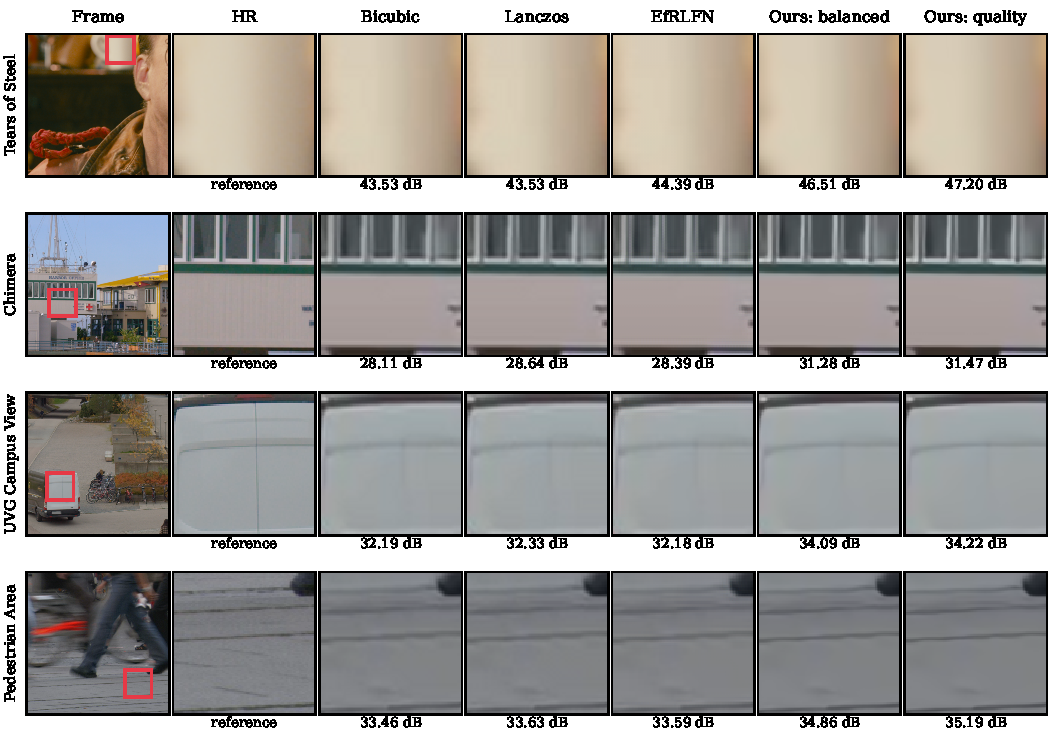
\includegraphics[width=\textwidth]{figures/visual.pdf}
  \caption{\textbf{Visual comparison} on held-out scenes, x264 CRF~26. For each scene the
  96$\times$96 crop (with detail) where \emph{quality} gains most over Lanczos was selected, so
  the crops show the best case, not a random sample. Luma models use bilinear chroma. PSNR-Y of
  the crop below each panel.}
  \label{fig:visual}
\end{figure*}

\paragraph{Speed vs quality.} \Cref{fig:tradeoff} plots the streaming-track gain against the
in-browser runtime at 1080p$\to$4K. \emph{balanced} and \emph{quality} are 42$\times$ and
12$\times$ faster than EfRLFN. Only they fit the 12\,ms budget that a 24\,fps film leaves
after decoding at 4K output.

\begin{figure}[t]
  \centering
  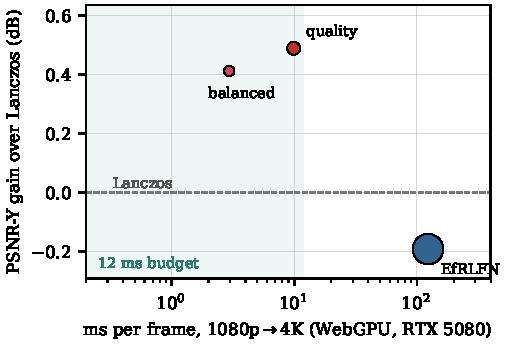
\includegraphics[width=\columnwidth]{figures/tradeoff.pdf}
  \caption{\textbf{Streaming PSNR-Y gain over Lanczos vs.\ runtime} (complete WebGPU chain,
  1080p$\to$4K, RTX~5080, log scale). Marker area $\propto$ parameters.}
  \label{fig:tradeoff}
\end{figure}

\begin{table}[t]
\centering
\caption{\textbf{In-browser runtime} (ms per frame, WebGPU, Chrome, RTX~5080, f16). CNN stage
alone / complete chain (deband, CNN, EASU if needed, RCAS, grain).}
\label{tab:runtime}
\resizebox{\columnwidth}{!}{%
\begin{tabular}{lcccc}
\toprule
Source $\to$ output & FSR~1 only & \emph{balanced} & \emph{quality} & EfRLFN \
\midrule
360p $\to$ 720p & 0.07 & 0.39 / 0.39 & 1.05 / 1.08 & 12.0 / 12.3 \
720p $\to$ 1440p & 0.13 & 1.25 / 1.31 & 4.06 / 4.13 & 53.9 / 54.2 \
1080p $\to$ 2160p & 0.39 & 2.75 / 2.95 & 9.70 / 9.90 & 123.0 / 123.4 \
720p $\to$ 2160p & 0.39 & 1.44 / 1.61 & 4.33 / 4.46 & 54.8 / 55.1 \
\bottomrule
\end{tabular}}
\end{table}


\section{Limitations}
\begin{itemize}
\setlength\itemsep{0pt}
\item \textbf{Clean, flat input.} On frames that interpolation already reproduces almost
perfectly, the networks lose up to 2\,dB (\cref{tab:flat}). Mixing more uncompressed pairs into
training, or a gate on the residual, should close this; neither is evaluated here.
\item \textbf{Smoothing.} The networks are PSNR-trained and smooth rather than hallucinate; the
plugin re-adds film grain afterwards, which our metrics do not reward.
\item \textbf{Chroma.} Chroma is only interpolated.
\item \textbf{Scale.} Only 2$\times$ is trained. A 720p$\to$4K view is upscaled 2$\times$ by the
network and the rest by EASU. Dedicated 3$\times$ models are future work.
\item \textbf{Metrics.} We report full-reference fidelity only. A perceptual study would be the
right test for the grain and sharpening stages.
\end{itemize}

\section{Conclusion}
For player-side upscaling of compressed live action, a 12k--48k parameter luma network trained
on real codec round-trips of permissively licensed footage gains about half a decibel PSNR-Y and
3 VMAF points over Lanczos on streaming-compressed input. It does so at a cost that fits
integrated GPUs, and it ships under MIT. On clean, flat input it does not beat Lanczos, which
marks where the next iteration should go. The weights, the training
pipeline, the data recipe and the browser runtime are available at
\url{https://github.com/PianoNic/LiveActionSR},
\url{https://huggingface.co/PianoNic/LiveActionSR-2x} and
\url{https://github.com/PianoNic/ArtPlayerPluginLiveActionSR}.

\paragraph{Acknowledgements.} Footage: Netflix Open Content (CC BY 4.0); \emph{Tears of Steel}, (CC)
Blender Foundation | mango.blender.org (CC BY 3.0); UVG-VCM, Ultra Video Group, Tampere University
(CC BY 4.0); TU München; SVT Sveriges Television. EfRLFN weights: MSU Graphics \& Media Lab (MIT).

\small
\begin{thebibliography}{99}
\bibitem{srcnn} C.~Dong, C.~C.~Loy, K.~He, X.~Tang. Learning a deep convolutional network for
image super-resolution. \emph{ECCV}, 2014.
\bibitem{fsrcnn} C.~Dong, C.~C.~Loy, X.~Tang. Accelerating the super-resolution convolutional
neural network. \emph{ECCV}, 2016.
\bibitem{espcn} W.~Shi et al. Real-time single image and video super-resolution using an efficient
sub-pixel convolutional neural network. \emph{CVPR}, 2016.
\bibitem{rlfn} F.~Kong et al. Residual local feature network for efficient super-resolution.
\emph{CVPR Workshops}, 2022.
\bibitem{span} C.~Wan et al. Swift parameter-free attention network for efficient
super-resolution. \emph{CVPR Workshops}, 2024.
\bibitem{ntire24} B.~Ren et al. The ninth NTIRE 2024 efficient super-resolution challenge report.
\emph{CVPR Workshops}, 2024.
\bibitem{efrlfn} E.~Bogatyrev, K.~Abud, I.~Molodetskikh, N.~Alutis, D.~Vatolin. Exploring
real-time super-resolution: benchmarking and fine-tuning for streaming content. \emph{ICLR}, 2026.
arXiv:2602.11339.
\bibitem{aim24} M.~V.~Conde et al. AIM 2024 challenge on efficient video super-resolution for
AV1 compressed content. arXiv:2409.17256, 2024.
\bibitem{bsrgan} K.~Zhang, J.~Liang, L.~Van~Gool, R.~Timofte. Designing a practical degradation
model for deep blind image super-resolution. \emph{ICCV}, 2021.
\bibitem{realesrgan} X.~Wang, L.~Xie, C.~Dong, Y.~Shan. Real-ESRGAN: training real-world blind
super-resolution with pure synthetic data. \emph{ICCV Workshops}, 2021.
\bibitem{eca} Q.~Wang et al. ECA-Net: efficient channel attention for deep convolutional neural
networks. \emph{CVPR}, 2020.
\bibitem{fsr} AMD. FidelityFX Super Resolution 1.0. GPUOpen, 2021.
\bibitem{anime4k} bloc97. Anime4K. \url{https://github.com/bloc97/Anime4K}.
\bibitem{artcnn} Artoriuz. ArtCNN. \url{https://github.com/Artoriuz/ArtCNN}.
\bibitem{netflixoc} Netflix. Open Content. \url{https://opencontent.netflix.com}.
\bibitem{uvgvcm} T.~Partanen et al. UVG-VCM: benchmarking dataset for machine-oriented visual data
compression. \emph{QoMEX}, 2026.
\bibitem{ssim} Z.~Wang, A.~C.~Bovik, H.~R.~Sheikh, E.~P.~Simoncelli. Image quality assessment:
from error visibility to structural similarity. \emph{IEEE TIP}, 13(4), 2004.
\end{thebibliography}

\end{document}
